\section{Introduction}
\label{sec:intro}

% infographics is useful
Infographics use a combination of graphics, text, images, and data to inform and engage.
In animated infographics, some elements are animated to illustrate data in a more exciting and engaging way or to emphasize key points.
% animated infographics are useful
The animation of infographics is considered a powerful tool for storytelling. 
It has been widely used in multiple areas, such as business, publicity, science popularization and so on. 
Compared to static infographics, it can interpret data or ideas in a more vivid way and grabs the audience's attention quickly, appreciated and shared by people for years~\cite{blazer2019animated, brehmer2016timelines}. % [5, 10] in "Communicating with Motion: A Design Space for Animated Visual Narratives in Data Videos"

% example
For instance, \autoref{fig:ani_example} illustrates a timeline and keyframes of an animated infographics video, which tries to explain the relationship between SAT score and family income.
In this animation, the chart framework enters at the beginning (A1) when the author explains this chart.
Different chart components will use different effects. For example, the lines use WipeIn effect while the x-label on the left use CutIn effect.
Following the narration, the bar and bar label for the category "less than \$20,000" enter (A2). A line and a label fade in to illustrate the average score (A3).
Then bars in the middle wipe in with a stagger (A4) in order to show a positive correlation.
Finally, the author introduces the data for "More than \$200,000" with similar effects on the corresponding bar and label (A5).
% Such animated infographics make audiences easy to follow the narration and complex data facts can be explained intuitively, appreciated and shared by people for years.

\begin{figure}[h]
  \centering
  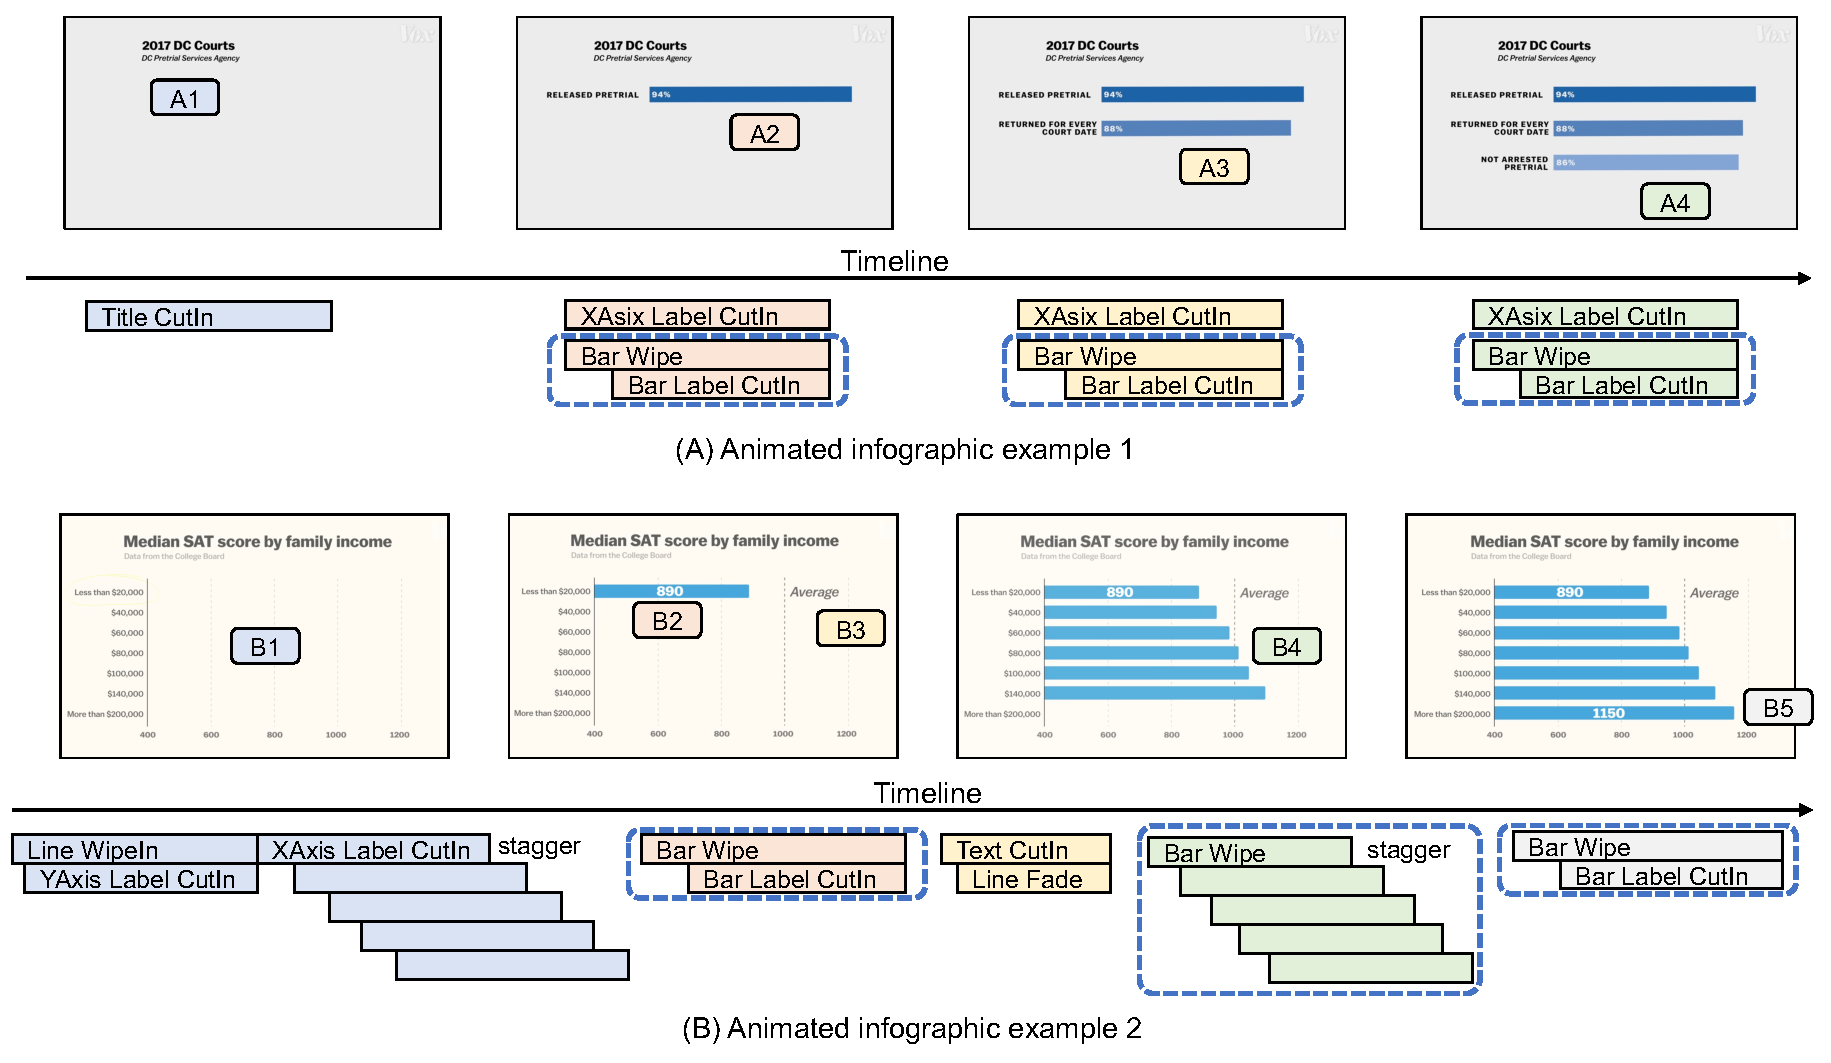
\includegraphics[width=\linewidth]{figs/ani_example.png}
  \caption{Animated infographics example (\url{https://youtu.be/WjVVwMGJ9S8?t=334}).}
  \Description{An animated infogrphics about the relation between SAT score and the family income}
  \label{fig:ani_example}
\end{figure}

% introduce existing approaches and shortcomes
Unfortunately, the creation of animated infographics is tedious and time-consuming, especially for novice users~\cite{amini2016authoring, hullman2013deeper, shi2021communicating}. %[5 dataclip, 41, 80, in Katika]
It can take weeks for authoring graphical animation itself that lasts around one minute \cite{howlong}.
% Cite these papers: “Recent works [5, 41, 80] illustrate how authoring a motion graphics video is a challenging task, and creating a minute-long video can take up to two days [71]”, in Katika
% how to create it in AI/AE
First, designers need to create static infographics (like \autoref{fig:ani_example}(D)) using some feature-rich softwares such as Adobe Illustrator~\cite{AdobeAI} or D3~\cite{bostock2011d3}.
Then they can export their infographics as Scalable Vector Graphics (SVG) or other kinds of files, so that downstream tools can be employed for animation creation.
Adobe After Effects~\cite{AdobeAE} is one of the most widely-used and powerful tools for this task because of its high expressiveness, which uses keyframes for creating.
Here we take the animations (A1-5) in \autoref{fig:ani_example} as an example.
Basically, each animation needs to: 
1) select animation target;
2) drag the playhead to create a start keyframe and set initial properties;
3) drag the playhead to create a end keyframe and set final properties;
4) specify an appropriate easing function.
% A1
To implement the enter effect of lines and labels in A1, each element needs to be masked separately.
Designers need to set the y coordinates of labels at the start/end keyframe to let them move out from the masks.
For lines, designers need to set the initial and final properties of masks.
% A2 A5
For animation A2 and A5, the wipe-in effect of the bar and cut-in effect of text is similar, but they will have a different direction.
% A3
Changing the initial opacity of the average line can implement animation A3.
% A4
Animation A4 requires the keyframes of each element to be set at a specified interval in order to achieve the stagger effect.
Because the keyframes and parameters are different across elements, similar operations will be performed multiple times.
% conclusion
Given this situation, though these existing tools are helpful, designers of animated infographics still take a procedural approach to creating them from scratch: draw the elements, select targets and apply animations one by one, as mentioned in the work of Thompson \etal~\cite{thompson2020understanding}.
%Besides, specifying visual properties is not an intuitive way for animation creation and requires expertise~\cite{}.

% Gaia
To facilitate the creation procedure,  declarative languages are typically preferred by users as they favor conciseness over expressiveness~\cite{mcnutt2023nogrammar}. 
In this work, we aim to reduce the burden of creating animated infographics greatly. 
We propose \gaia{}, a declarative Grammar for animated infographics. 
It has 3 major features. 
The first one is \textbf{expressivity}: \gaia{} is both expressive and intuitive for reading and writing.
In \gaia{}, animations are represented by effects applied to a group of visual elements instead of a set of keyframes.
% insight: hierarchy of components and animations
We refer one infographic as an instance, and groups of elements as components.
Components in one instance form a hierarchy and each component can apply effects as a group.
Besides, grouping is also a way to organize animations~\cite{thompson2020understanding}. Animations for components can be combined with several alignment strategies, which also form a hierarchical structure. 
% Gaia
\gaia{} provides a declarative grammar following these insights, which enables designers to create animations for components and organize them in a hierarchical timeline.
In this way, \gaia{} can support flexible and intuitive animation creation for infographics and can express complex animation timelines easily.
Meanwhile, a wider variety of components (not limited to marks) can also be animated using \gaia{}.

The second feature is \textbf{reusability}: \gaia{} spec can be used as infographic animation templates.
% insight: animations share similarity
This is motivated by our observations that animations share similarities, such as entering animations of axes existing in many animated chart videos. 
Animation A2 and A5 in \autoref{fig:ani_example}, as another example, can be extracted and reused, or even on other bar chart instances.
As mentioned by Thompson \etal~\cite{thompson2020understanding}, reusing animations on similar components in one or across multiple instances is useful, which simplifies and speeds up the creation process.
% Gaia
To this end, we conduct a target abstraction to describe graphical elements in infographics. 
The animations are not directly bound to the graphical elements but instead, bind to the role of the elements. 
Via this mechanism, \gaia{} keeps the type information about animated components. 
For instance, \gaia{} can recognize different types of animated elements in axis components, such as domain, ticks and labels.
A wide range of SVGs from the internet or other design tools can be converted to structure-awared SVG (SSVG) through semantic binding, which contains the roles of each animated target and other information (like data). 
By taking SSVG files as input, users can reuse animations from themselves or other designers.

The last feature is \textbf{extensibility}: Templates in \gaia{} can be extended.
% insight
Existing declarative languages only provide a few common effects like fade and wipe.
Meanwhile, these techniques don’t provide support for extending the animation library. The only way to do this is through a code-level implementation.
% Gaia
Based on the target abstraction and modularity, \gaia{} allows users to define new templates through the same declarative grammar as animation creation without relying on a concrete instance, then add them to the library and use them just as other existing templates. 
For example, users can combine templates for bars and axes to create a new template for bar charts. 
Parameter abstraction is also introduced in \gaia{} so that a template can be more generic and customizable.

We implemented a \gaia{} interpreter prototype and packaged it as a TS library.
Through a demo system with a variety of examples, we show the usability of \gaia{}. Our examples include: 1) reproduced animations with narration taken from existing animation videos; 2) animations used in other declarative animation creation language.
Compared to existing language, we showed that \gaia{} is more expressive and intuitive.
According to the result of the user study, \gaia{} obtained good feedback from users.

In brief, the main contributions of this work include:
\begin{enumerate}
\item \textbf{A set of high-level grammars} that enables intuitive creation of animations. 
Users can build complex animations via a hierarchical view and concatenating operations. 
Abstraction mechanisms, such as target type abstraction, enable reusability and extendability of \gaia{}, which is the first attempt for declarative animation grammars.
\item \textbf{An animation interpreter engine} and \textbf{a demo system} with multiple examples.
\item \textbf{An evaluation} on the usability of \gaia{} with non-experts in animation design.
\end{enumerate}